% Cislunar electric cargo tug: Phase 0/A-style study report
% Build from this folder:  latexmk -pdf cislunar-tug-study-report.tex
% Figures: python report/figures/make_figures.py (run from the repository root)
\documentclass[11pt,a4paper]{article}

% ------------------------------------------------------------------ settings
\newcommand{\studyauthor}{Robert Custron}
\newcommand{\studydate}{October 2026}
\newcommand{\repourl}{https://github.com/Robertcustron/cislunar-tug-study}
% ------------------------------------------------------------------ packages
\usepackage[T1]{fontenc}
\usepackage[utf8]{inputenc}
\usepackage{mathptmx}                 % Times text and maths
\usepackage[scaled=0.92]{helvet}      % Helvetica for headings
\usepackage{courier}
\usepackage[a4paper,top=25mm,bottom=25mm,left=25mm,right=25mm,headheight=14pt]{geometry}
\usepackage{microtype}
\usepackage{graphicx}
\usepackage[table]{xcolor}
\usepackage{booktabs,tabularx,array,longtable,multirow}
\usepackage[labelsep=colon,skip=6pt]{caption}
\usepackage{enumitem}
\usepackage{titlesec}
\usepackage{fancyhdr}
\usepackage{tcolorbox}
\usepackage{amsmath}
\usepackage{textcomp}
\usepackage{rotating}
\usepackage[colorlinks=true,linkcolor=black,citecolor=black,urlcolor=blue]{hyperref}
\usepackage{xurl}
\urlstyle{same}
\usepackage{float}
\usepackage[capitalise,nameinlink]{cleveref}

\definecolor{panel}{gray}{0.94}
\definecolor{rule}{gray}{0.6}

\setlength{\parindent}{0pt}
\setlength{\parskip}{6pt plus 1pt}
\renewcommand{\arraystretch}{1.15}
\setlist{nosep,leftmargin=1.4em,topsep=3pt}
\newcolumntype{L}{>{\raggedright\arraybackslash}X}
\newcolumntype{P}[1]{>{\raggedright\arraybackslash}p{#1}}

\titleformat{\section}{\sffamily\Large\bfseries}{\thesection}{0.8em}{}
\titleformat{\subsection}{\sffamily\large\bfseries}{\thesubsection}{0.8em}{}
\titleformat{\paragraph}[runin]{\normalfont\bfseries}{}{}{}[.]
\titlespacing*{\section}{0pt}{18pt}{8pt}
\titlespacing*{\subsection}{0pt}{12pt}{4pt}
\titlespacing*{\paragraph}{0pt}{6pt}{0.6em}

% Running head as in the thesis template: "Section | page"
\pagestyle{fancy}
\fancyhf{}
\renewcommand{\sectionmark}[1]{\markboth{#1}{}}
\fancyhead[R]{\sffamily\small\nouppercase{\leftmark}\,\textbar\,\thepage}
\renewcommand{\headrulewidth}{0pt}
\fancypagestyle{plain}{\fancyhf{}\fancyhead[R]{\sffamily\small\thepage}\fancyfoot[C]{\footnotesize\itshape Personal learning study, not for professional use}\renewcommand{\headrulewidth}{0pt}}

\newtcolorbox{keybox}[1]{colback=panel,colframe=panel,sharp corners,boxrule=0pt,left=4mm,right=4mm,top=3mm,bottom=3mm,
  fonttitle=\bfseries,coltitle=black,title={#1},colbacktitle=panel,toptitle=1mm,bottomtitle=-1mm}
\newtcolorbox{noticebox}{colback=panel,colframe=black,sharp corners,boxrule=0.5pt,left=4mm,right=4mm,top=3mm,bottom=3mm}

\newcommand{\figsrc}[1]{\par\vspace{2pt}{\raggedright\footnotesize #1\par}}
\newcommand{\id}[1]{#1}

% Capella diagram exports (vector PDF in figures/capella/)
\newcommand{\capellafig}[3]{% file name, caption, label
  \begin{figure}[htbp]\centering
  \includegraphics[width=\linewidth,height=0.42\textheight,keepaspectratio]{capella/#1.pdf}
  \caption{#2}\label{#3}\end{figure}}

\graphicspath{{figures/}}

% ------------------------------------------------------------------ document
\begin{document}

% ---------------- title page
\begin{titlepage}
\thispagestyle{empty}
\centering
\vspace*{40mm}
{\sffamily Phase 0/A-style systems engineering study\par}
\vspace{2mm}
{\sffamily\small Personal learning project\par}
\vspace{14mm}
{\sffamily\bfseries\fontsize{24}{30}\selectfont A Reusable, Refuellable\\ Solar-Electric Cargo Tug\\ between Earth Orbit and the Moon\par}
\vspace{10mm}
{\sffamily\bfseries\MakeUppercase{\studyauthor}\par}
\vspace{6mm}
{\large Mission definition, operational and system analysis, requirements flow-down,\\ trade-offs, logical architecture, and TRL and cost assessment\par}
\vfill
\begin{noticebox}
\textbf{Personal learning study, not for professional use.}\par\smallskip
\small This report is the result of a self-directed learning project. It is not commissioned, reviewed or endorsed by ESA or by any company, uses public information only, and must not be used as a basis for engineering, programme or investment decisions. See ``About this study'' on the next page.
\end{noticebox}
\vspace{8mm}
{\small
\begin{tabular}{@{}ll}
Date & \studydate \\
Methods & Arcadia in Capella and Python \\
Repository & \url{\repourl}\\
\end{tabular}\par}
\end{titlepage}


% ---------------- about + summary
\section*{About this study}
\addcontentsline{toc}{section}{About this study}
\markboth{About this study}{}

\textbf{Why it exists.} I made this study to learn how an early-phase space mission study is actually done, by doing one from the beginning. I started from ESA's own long-term strategy documents, \emph{ESA Strategy 2040}~\cite{strategy2040}, \emph{Explore2040}~\cite{explore2040} and the \emph{Technology Vision 2040}~\cite{techvision}, analysed what they ask for, and developed a mission study that is aligned with that vision: a reusable, refuellable electric cargo tug for the ``hub-and-spoke'' space logistics the strategy calls for. Along the way I worked through each Phase 0/A activity in turn: mission definition, operational analysis, system analysis with a requirements flow-down, trade-offs, a logical architecture, and a technology readiness (TRL) and cost-driver assessment. The modelling uses the Arcadia method in Capella, and the numbers come from a small, tested Python model.

\textbf{What it is not.} This is not a professional or industrial study, and it should not be used as one.
\begin{itemize}
  \item It has not been commissioned, reviewed or endorsed by ESA, by any space agency or by any company, and it is not affiliated with any of them.
  \item It uses public information only (the documents and papers in the references) and no information from any employer.
  \item Every number is either taken from a cited public source or is my own estimate, stated as an assumption (Appendix~\ref{app:registers}). Many are deliberately simple, and none has been validated by test or by independent review.
  \item The results must not be used as a basis for engineering, programme, procurement or investment decisions. Views and conclusions are my own.
\end{itemize}

\textbf{How to read it.} Each section summarises one phase of the study; the full work is in the repository~\cite{repo}, where every requirement, assumption (\id{A-}), decision (\id{D-}) and calculation (\id{CALC-}) has an identifier, so any number in this report can be traced to its source. Values marked TBD are not yet set; TBC means set but to be confirmed.

\begin{keybox}{Summary of results}
\small
\begin{itemize}[leftmargin=1.1em]
  \item \textbf{Concept.} A 25~kW solar-electric tug carries 5~t of cargo from a GTO-class staging orbit to the near-rectilinear halo orbit (NRHO) around the Moon and returns, 9 times in a 15-year life (1.5-year round trip). It is refuelled each trip with 2.5~t of xenon from a passive module launched together with the cargo on one Ariane~64.
  \item \textbf{Requirements.} 26 system requirements, 14 subsystem requirements for propulsion, power and the docking and refuelling interface, and 8 interface requirements, each traced up to a mission objective, assumption or calculation and down to logical components.
  \item \textbf{Trade-offs.} 25~kW gives 9 trips with a 12\,\% power margin and matches five European 5~kW thrusters plus a spare. Fluid transfer from a co-launched module is the most robust refuelling concept.
  \item \textbf{Main finding.} Whatever the power, the tug thrusts for about 90,000~h over its life, against 15,000--20,000~h of rated life for today's European thruster. Thruster life, not power or propellant, limits reuse.
  \item \textbf{TRL and cost.} Five critical technologies sit at TRL 3--5 for this application. The bottom-up dry mass with ESA margins is 4.65~t against a 6.08~t parametric baseline. The largest cost driver is one launch per trip: at 5~t per trip the tug needs 10 launches where direct delivery needs 7; at about 7~t per trip the gap falls to one launch.
\end{itemize}
\end{keybox}

\newpage
{\small\tableofcontents}
\vspace{4pt}
% =====================================================================

\newpage
\section{Introduction}

\paragraph{Objective} Define a minimal but credible concept for a reusable, refuellable cargo tug between Earth orbit and the Moon, and work it through the systems engineering activities of a Phase 0/A study: from the stakeholder need to requirements, to a justified design point, to an architecture, and finally to the technologies and costs that decide whether the concept is worth pursuing.

\paragraph{Approach} The study follows the Arcadia method~\cite{arcadia} with its model in Capella: operational analysis (what stakeholders need, without the tug), system analysis (the tug as a black box with functions, interfaces, modes and requirements) and logical architecture (the tug split into components). Quantitative work is done in a Python model~\cite{repo}; it computes the transfers with the rocket equation, sweeps power, sizes the power chain and builds the mass budget. Requirements are kept in traceability tables (CSV files) alongside the model. The repository holds the phase documents, the Capella model and the full calculation log, so each step can be followed in more detail. Table~\ref{tab:phases} maps each phase to its outputs. 

\begin{table}[htbp]\centering\small
\caption{Study phases and their main outputs.}\label{tab:phases}
\begin{tabularx}{\linewidth}{@{}P{3.4cm}LP{2.6cm}@{}}
\toprule
Phase & Main outputs & Section \\
\midrule
Mission definition & Mission statement, objectives, constraints, flight mechanics, assumptions & \ref{sec:mission} \\
Operational analysis & 7 entities, 5 capabilities, 20 activities, round-trip scenario (Capella) & \ref{sec:oa} \\
System analysis & Functions, exchanges, functional chains, modes; 26 system and 14 subsystem requirements & \ref{sec:sa} \\
Trade-offs & Power level vs transfer time (quantitative), refuelling concept (weighted scoring) & \ref{sec:trades} \\
Logical architecture & 8 components, 20 interfaces, 8 interface requirements, power budget & \ref{sec:la} \\
TRL and cost assessment & 5 critical technologies, bottom-up mass budget, thruster life strategy, cost drivers & \ref{sec:trl} \\
\bottomrule
\end{tabularx}
\end{table}

% =====================================================================
\section{Mission definition}\label{sec:mission}

\paragraph{Strategic premise} The concept is the premise of the study, not a result: it is drawn from ESA's 2040 documents. Strategy~2040 calls for a ``scalable `Hub-and-Spoke' network approach for space logistics through new launchers and space tugs'' and for in-orbit refuelling and servicing technologies~\cite[p.~45]{strategy2040}. Explore2040 expects electric propulsion tugs to ``lower the costs, leading to more frequent missions carrying ever larger payloads''~\cite[p.~16]{explore2040}, and the Technology Vision names very-high-power electric propulsion for large cargo missions and modular, reusable systems~\cite[pp.~45, 50]{techvision}. The study therefore asks \emph{how} such a tug should be built, and judges it against the simplest alternative: launching the cargo directly to the Moon (\id{D-09}).

\paragraph{Mission statement} \emph{Transport 5,000~kg of cargo per trip from a GTO-class Earth staging orbit to the Earth--Moon NRHO with an autonomous, reusable and refuellable solar-electric tug, repeatedly over a 15-year life, as part of a European hub-and-spoke logistics architecture.}

\begin{table}[htbp]\centering\small
\caption{Mission objectives.}\label{tab:mo}
\begin{tabularx}{\linewidth}{@{}P{1.1cm}P{3.2cm}L@{}}
\toprule
ID & Objective & Success criterion \\
\midrule
\id{MO-1} & Primary transport & 5,000~kg of net cargo delivered to NRHO per outbound trip \\
\id{MO-2} & Return cargo & Up to 500~kg returned per trip to the staging orbit (optional) \\
\id{MO-3} & Reuse and refuelling & 15-year design life, refuelled in Earth orbit; trip count set by the power trade-off \\
\id{MO-4} & European non-dependence & Ariane~6 launch; critical subsystems sourced in Europe \\
\id{MO-5} & Zero Debris disposal & Heliocentric disposal via lunar flyby, or controlled lunar impact \\
\bottomrule
\end{tabularx}
\end{table}

\paragraph{Baseline choices} Four decisions shape everything that follows.
\begin{itemize}
  \item \textbf{Staging orbit: GTO-class} (\id{D-02}). A start from low Earth orbit roughly doubles the low-thrust delta-v (about 6~km/s from LEO to GEO alone~\cite{loghry}). SMART-1, a published reusable tug design and Gateway's power and propulsion element all start from GTO-class orbits~\cite{estublier,rimani,mcguire2024}.
  \item \textbf{Destination: NRHO} (\id{D-03}, \id{D-10}). It is reached for 2.4--3.1~km/s, costs about 10~m/s per year to maintain and avoids long eclipses~\cite{whynrho}. Low lunar orbit is excluded: it adds about 1.6~km/s per leg and long eclipses, and descent belongs to the lander. NASA paused Gateway in March 2026~\cite{gatewaypause}, so NRHO is treated as a staging orbit, not a Gateway commitment.
  \item \textbf{Propulsion: Hall thrusters on xenon} (\id{D-04}), at 2,100~s and 60\,\% efficiency, with the thrusters off in eclipse and an 85\,\% thrusting duty cycle (\id{A-17}, \id{A-19}).
  \item \textbf{Delta-v: 2.4~km/s per leg plus a 10\,\% margin, 2.64~km/s} (\id{A-06}), from a published GTO-to-NRHO tug design~\cite{rimani}; 3.1~km/s, the Gateway transfer~\cite{mcguire2024}, is the sensitivity case.
\end{itemize}

Each round trip uses one Ariane~64 (11.5~t to GTO~\cite{ariane}) for the cargo and the next trip's propellant (\id{A-09}). Figure~\ref{fig:concept} shows the resulting round trip at the design point chosen in the trade-offs.

\begin{figure}[htbp]\centering
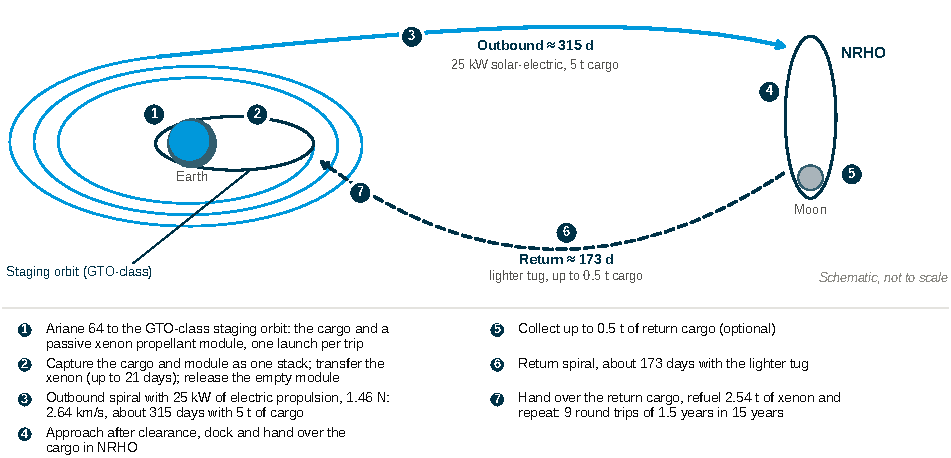
\includegraphics[width=\linewidth]{fig01_mission_concept.pdf}
\caption{Concept of operations at the design point (25~kW). Durations from the model at 5~t outbound and 0.5~t return cargo.}\label{fig:concept}
%\figsrc{Source: \texttt{model/results/baseline/power\_trade.csv} (25~kW row).}
\end{figure}

% =====================================================================
\section{Operational analysis}\label{sec:oa}

In Arcadia the operational analysis describes what the stakeholders need to achieve, not the solution, so the tug does not appear in it. Its place is taken by an entity called \emph{Cislunar Cargo Transport}: the need to move cargo and propellant between Earth and lunar orbit, however it is met (\id{D-06}). Seven operational entities take part: the cargo customer, the launch service provider, the cislunar cargo transport, ground operations, the lunar orbit destination, a propellant supplier and the space safety authority.

Five capabilities structure the need. An umbrella capability, \emph{provide reusable cislunar cargo logistics}, includes delivery to lunar orbit, propellant replenishment in orbit and safe disposal; with cargo return as an optional extension (\id{D-08}). The stakeholder need was written as ``replenish transport propellant in orbit'' rather than ``refuel the tug'' (\id{D-07}), the need left trade-offs open among a depot, tanker, and tank swap.. Twenty activities and nineteen interactions (seven physical, twelve information) connect the entities (Figure~\ref{fig:oab}), and one scenario walks through a complete round trip in fifteen messages.

\begin{figure}[htbp]\centering
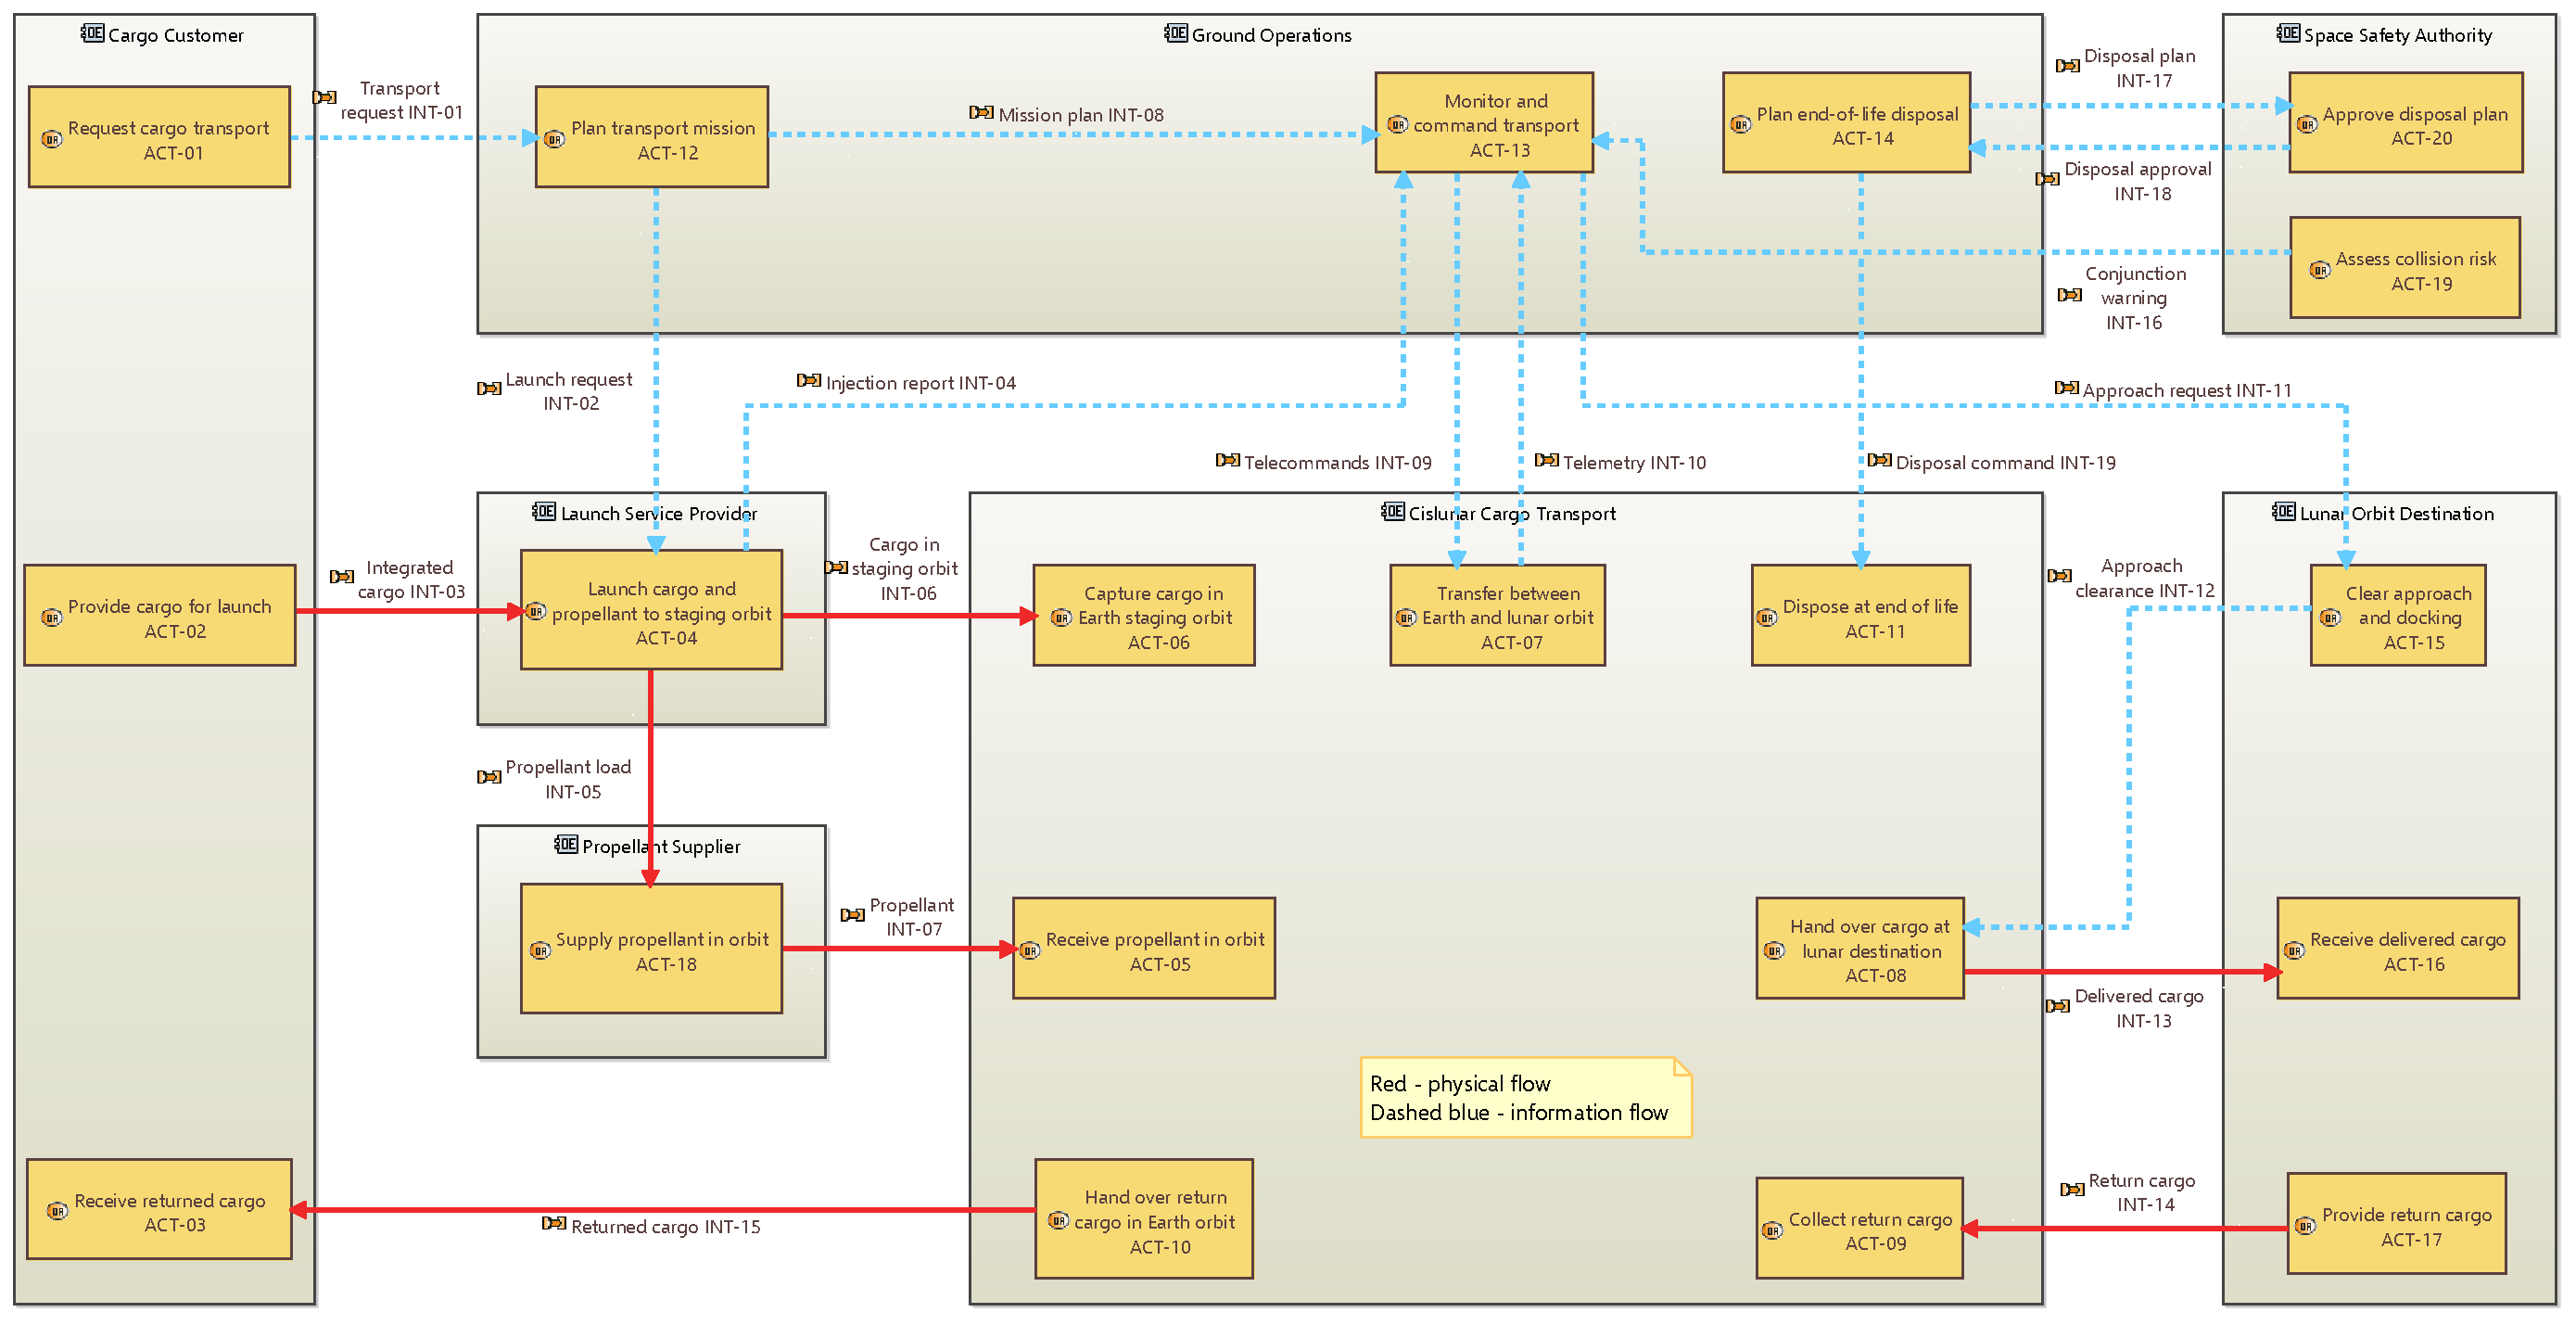
\includegraphics[width=\linewidth]{capella/OA-2_OAB.pdf}
\caption{Operational Architecture Blank, exported from the Capella model. Red: physical interactions (cargo, propellant); dashed blue: information. The tug is represented by the \emph{Cislunar Cargo Transport} entity.}\label{fig:oab}
\end{figure}

% =====================================================================
\section{System analysis and requirements}\label{sec:sa}

\paragraph{Boundary} The cislunar cargo transport becomes the System, the \emph{Cislunar Cargo Tug}. Everything that exchanges something with it directly becomes an actor: the ground segment, the launch vehicle, the propellant supplier (later the propellant module), the lunar orbit destination, the cargo customer and the Sun, modelled as an actor to make the power chain and the eclipse requirement explicit (\id{A-20}). The ground segment is outside the boundary (\id{D-11}), and the space safety authority acts only through the ground (\id{D-12}).

\paragraph{Functions, chains and modes} The seven activities of the transport entity become seven top-level system functions; transfer and disposal are broken down, giving 17 leaf functions connected by 24 functional exchanges. Three functional chains carry the end-to-end paths that requirements anchor to: cargo capture and transfer, refuelling, and end-of-life disposal. A state machine defines seven modes (launch, commissioning, transfer, docking, refuelling, safe, disposal), later reused for the power budget. The Capella diagrams of this layer are in Appendix~\ref{app:capella} (Figures~\ref{fig:sa1} to~\ref{fig:sa4}).

\paragraph{Requirements} The system has 26 requirements in six groups: mission and performance, propulsion and refuelling, power and environment, proximity operations and interfaces, command and autonomy, and disposal and programmatics. Each has a source it traces to, the leaf functions it is allocated to and a verification method. The nine preliminary requirements of the mission definition are absorbed into this set. As the study scope specifies, three subsystems receive a flow-down: electric propulsion (\id{PROP}), electrical power (\id{PWR}) and the docking and refuelling interface (\id{DRI}), the three that carry the critical technologies (\id{D-14}). Figure~\ref{fig:flowdown} shows the current flow-down; Table~\ref{tab:keyreq} lists the requirements that drive the design.

\begin{figure}[htbp]\centering
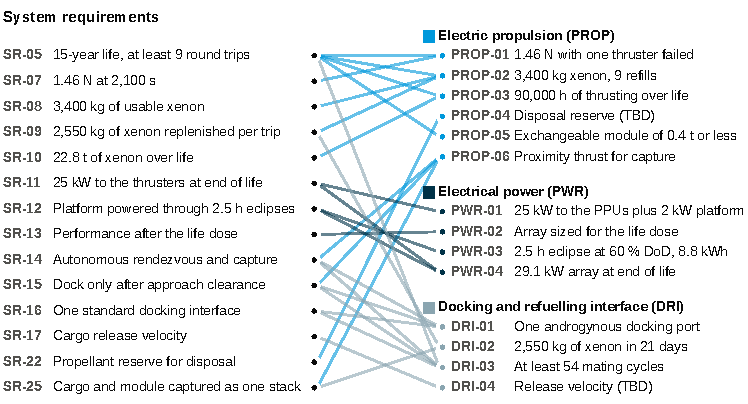
\includegraphics[width=\linewidth]{fig02_flowdown.pdf}
\caption{Flow-down from system to subsystem requirements. Each line is a ``derived from'' link in the requirement tables; labels are shortened.}\label{fig:flowdown}
\end{figure}

\begin{table}[htbp]\centering\small
\caption{Design-driving requirements, with their current values. ``Changed in'' shows the phase that set or revised the value.}\label{tab:keyreq}
\begin{tabularx}{\linewidth}{@{}P{1.6cm}LP{2.55cm}@{}}
\toprule
ID & Requirement (shortened) & Changed in \\
\midrule
\id{SR-01} & Transport at least 5,000~kg per round trip from a GTO-class orbit to NRHO & -- \\
\id{SR-05} & Design life of 15 years and at least 9 round trips & Trade-offs \\
\id{SR-07} & Total thrust of at least 1.46~N at a specific impulse of at least 2,100~s & Trade-offs \\
\id{SR-09} & Accept at least 2,550~kg of xenon in orbit per round trip & Trade-offs \\
\id{SR-11} & At least 25~kW to the electric propulsion at end of life, plus platform loads & Trade-offs \\
\id{SR-12} & Platform powered through eclipses of up to 2.5~h; longer ones avoided by trajectory design & Logical architecture \\
\id{SR-24} & Propulsion, power processing, arrays, GNC software and docking interfaces from European industry & -- \\
\id{SR-25} & Capture the cargo and its propellant module as one stack in a single rendezvous & Trade-offs \\
\id{PROP-03} & At least 90,000~h of thrusting over life (22.8~t of xenon); no qualified thruster meets it & Trade-offs \\
\id{PROP-05} & Thruster strings grouped in one exchangeable propulsion module of at most 0.4~t & TRL and cost \\
\id{PWR-03} & Battery carries the 2~kW platform through 2.5~h eclipses at 60\,\% depth of discharge (8.8~kWh) & Logical architecture \\
\id{DRI-03} & Docking and refuelling interface withstands at least 54 mating cycles & Trade-offs \\
\bottomrule
\end{tabularx}
\end{table}

The most useful result of the system analysis was the propulsion throughput requirement (\id{PROP-03}). Expressing life in processed xenon showed that the thrusters, not power or propellant, may be what limits reuse. That question was carried into both the trade-offs and the TRL assessment.

% =====================================================================
\section{Trade-offs}\label{sec:trades}

\subsection{Power level versus transfer time}

\paragraph{Method} The design variable is the electric power at the inputs of the power processing units (PPUs), swept from 12 to 48~kW. Thrust follows from $T = 2\eta P / (g_0 I_{sp})$; the dry mass grows by 25~kg per extra kW above 18~kW (\id{A-23}); the propellant per trip comes from the rocket equation worked backwards from the end of the return leg; leg time is propellant times exhaust velocity divided by thrust and duty cycle; and only whole round trips count in the 15-year life. Thruster wear is counted in firing hours for two thruster classes.

\begin{figure}[htbp]
\begin{minipage}[t]{0.47\linewidth}\vspace{0pt}\centering
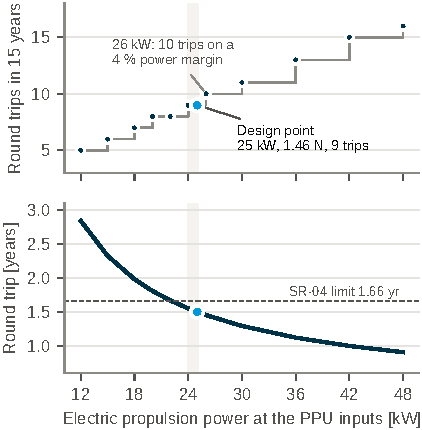
\includegraphics[width=\linewidth]{fig03_power_trade.pdf}
\captionof{figure}{Round trips in 15 years and round-trip time against electric propulsion power. The shaded band is the 24--25~kW pair of thruster options.}\label{fig:power}
\end{minipage}\hfill
\begin{minipage}[t]{0.5\linewidth}\vspace{0pt}\small
\captionof{table}{Trip count sensitivity, one parameter at a time.}\label{tab:sens}
\begin{tabularx}{\linewidth}{@{}Lrr@{}}
\toprule
Case & 18~kW & 25~kW \\
\midrule
Baseline & 7 & 9 \\
10\,\% less power & 6 & 9 \\
Specific mass 15~kg/kW & 7 & 10 \\
Specific mass 40~kg/kW & 7 & 9 \\
End operations 120 instead of 60~days & 6 & 9 \\
Delta-v 3.1~km/s per leg & 5 & 7 \\
$I_{sp}$ 1,800~s & 8 & 11 \\
\bottomrule
\end{tabularx}
\par\medskip
Throughput rises almost in step with power, because the transfer legs shrink as $1/P$ and only the 60 days of end operations are fixed. Neither the tug launch (8.6~t at 25~kW) nor the resupply launch comes near the 11.5~t Ariane~64 limit, so physics alone would keep pushing the power up. Cost, launch cadence and the power class of European hardware stop it.
\end{minipage}
\end{figure}

\paragraph{Decision} \textbf{25~kW, 1.46~N at 2,100~s} (\id{D-16}): a 1.50-year round trip and 9 trips, with a 12\,\% power margin on the ninth trip. The trip count is a step function, so the design point was chosen inside a step rather than at its edge: 18~kW, the mission definition reference, loses a trip with 10\,\% less power, and 26~kW gives a tenth trip on a 4\,\% margin that normal array degradation would remove. 25~kW is also exactly five European 5~kW-class thrusters at their nominal point, plus one spare in rotation (\id{D-20}); two 12~kW-class units at 24~kW are kept as the option.

\paragraph{Main finding} A faster tug finishes each trip sooner and then flies more trips, so the total thrusting time over 15 years barely changes with power: about 90,000~hours. With 5+1 units in rotation each thruster fires about 75,000~h, five times the rated life of the European 5~kW class; the mission uses about 30 rated thruster lifetimes however they are shared. Power cannot fix this, which made thruster wear-out the top risk for the TRL assessment (\id{D-18}).

\subsection{Refuelling concept}

Every trip the tug needs about 2.5~t of xenon back in the staging orbit. Four concepts were scored against seven weighted criteria, with a written reason for every score (Table~\ref{tab:refuel}). The decisive criterion is the maturity of the critical interface: xenon transfer couplers were developed and ground-tested in Europe for the Gateway ESPRIT refuelling module~\cite{ohbesprit,radke}, while no tank-module swap of this size, xenon depot or in-orbit 25~kW connector has been demonstrated.

\begin{table}[htbp]\centering\small
\caption{Refuelling concepts: weighted score (1 worst, 5 best) under six weight sets. Bold: first place.}\label{tab:refuel}
\begin{tabularx}{\linewidth}{@{}Lcccc@{}}
\toprule
Weight set & R1 Fluid transfer from & R2 Tank- & R3 Depot in & R4 Propulsion- \\
 & co-launched module & module swap & staging orbit & module swap \\
\midrule
Baseline & \textbf{2.90} & 2.80 & 2.60 & 2.75 \\
Equal weights & 2.86 & 2.86 & 2.86 & \textbf{3.00} \\
Maturity first & \textbf{3.15} & 2.90 & 2.60 & 2.65 \\
Cost first & \textbf{2.95} & 2.90 & 2.60 & 2.45 \\
Thruster life first & 2.40 & 2.30 & 2.30 & \textbf{3.25} \\
Sustainability first & 2.75 & 2.65 & \textbf{3.15} & 2.70 \\
\bottomrule
\end{tabularx}
\end{table}

\paragraph{Decision} \textbf{R1, fluid transfer from a passive propellant module launched with each cargo} (\id{D-17}). It ranks first under three weight sets and second under the other three (tied with R2 and R3 under equal weights); the scores are close, so the choice rests on robustness and on the most mature, European-built interface rather than on the arithmetic. A side benefit: the cargo and its xenon arrive as one stack, so one rendezvous per trip does both jobs (\id{SR-25}). Two options are kept on purpose: the propulsion-module swap (R4) as the answer to thruster wear, and the depot (R3) as the path into a wider logistics network, since it would use the same coupling.

% =====================================================================
\section{Logical architecture}\label{sec:la}

The logical architecture opens the black box. The tug is split into eight logical components (Figure~\ref{fig:la}). Propulsion, power and the docking and refuelling interface keep the boundaries of the flowed-down subsystems, so the flow-down stays valid (\id{D-21}). Thermal control and structure appear for the first time, because heat rejection and load paths only exist once there is a design. Every leaf function is allocated to exactly one component; three system functions that spanned two components were split, and two design-induced functions were added (heat rejection, launcher interface). The TRL and cost assessment later added one more, proximity thrust, giving 23 logical functions in total.

\begin{sidewaysfigure}
\centering
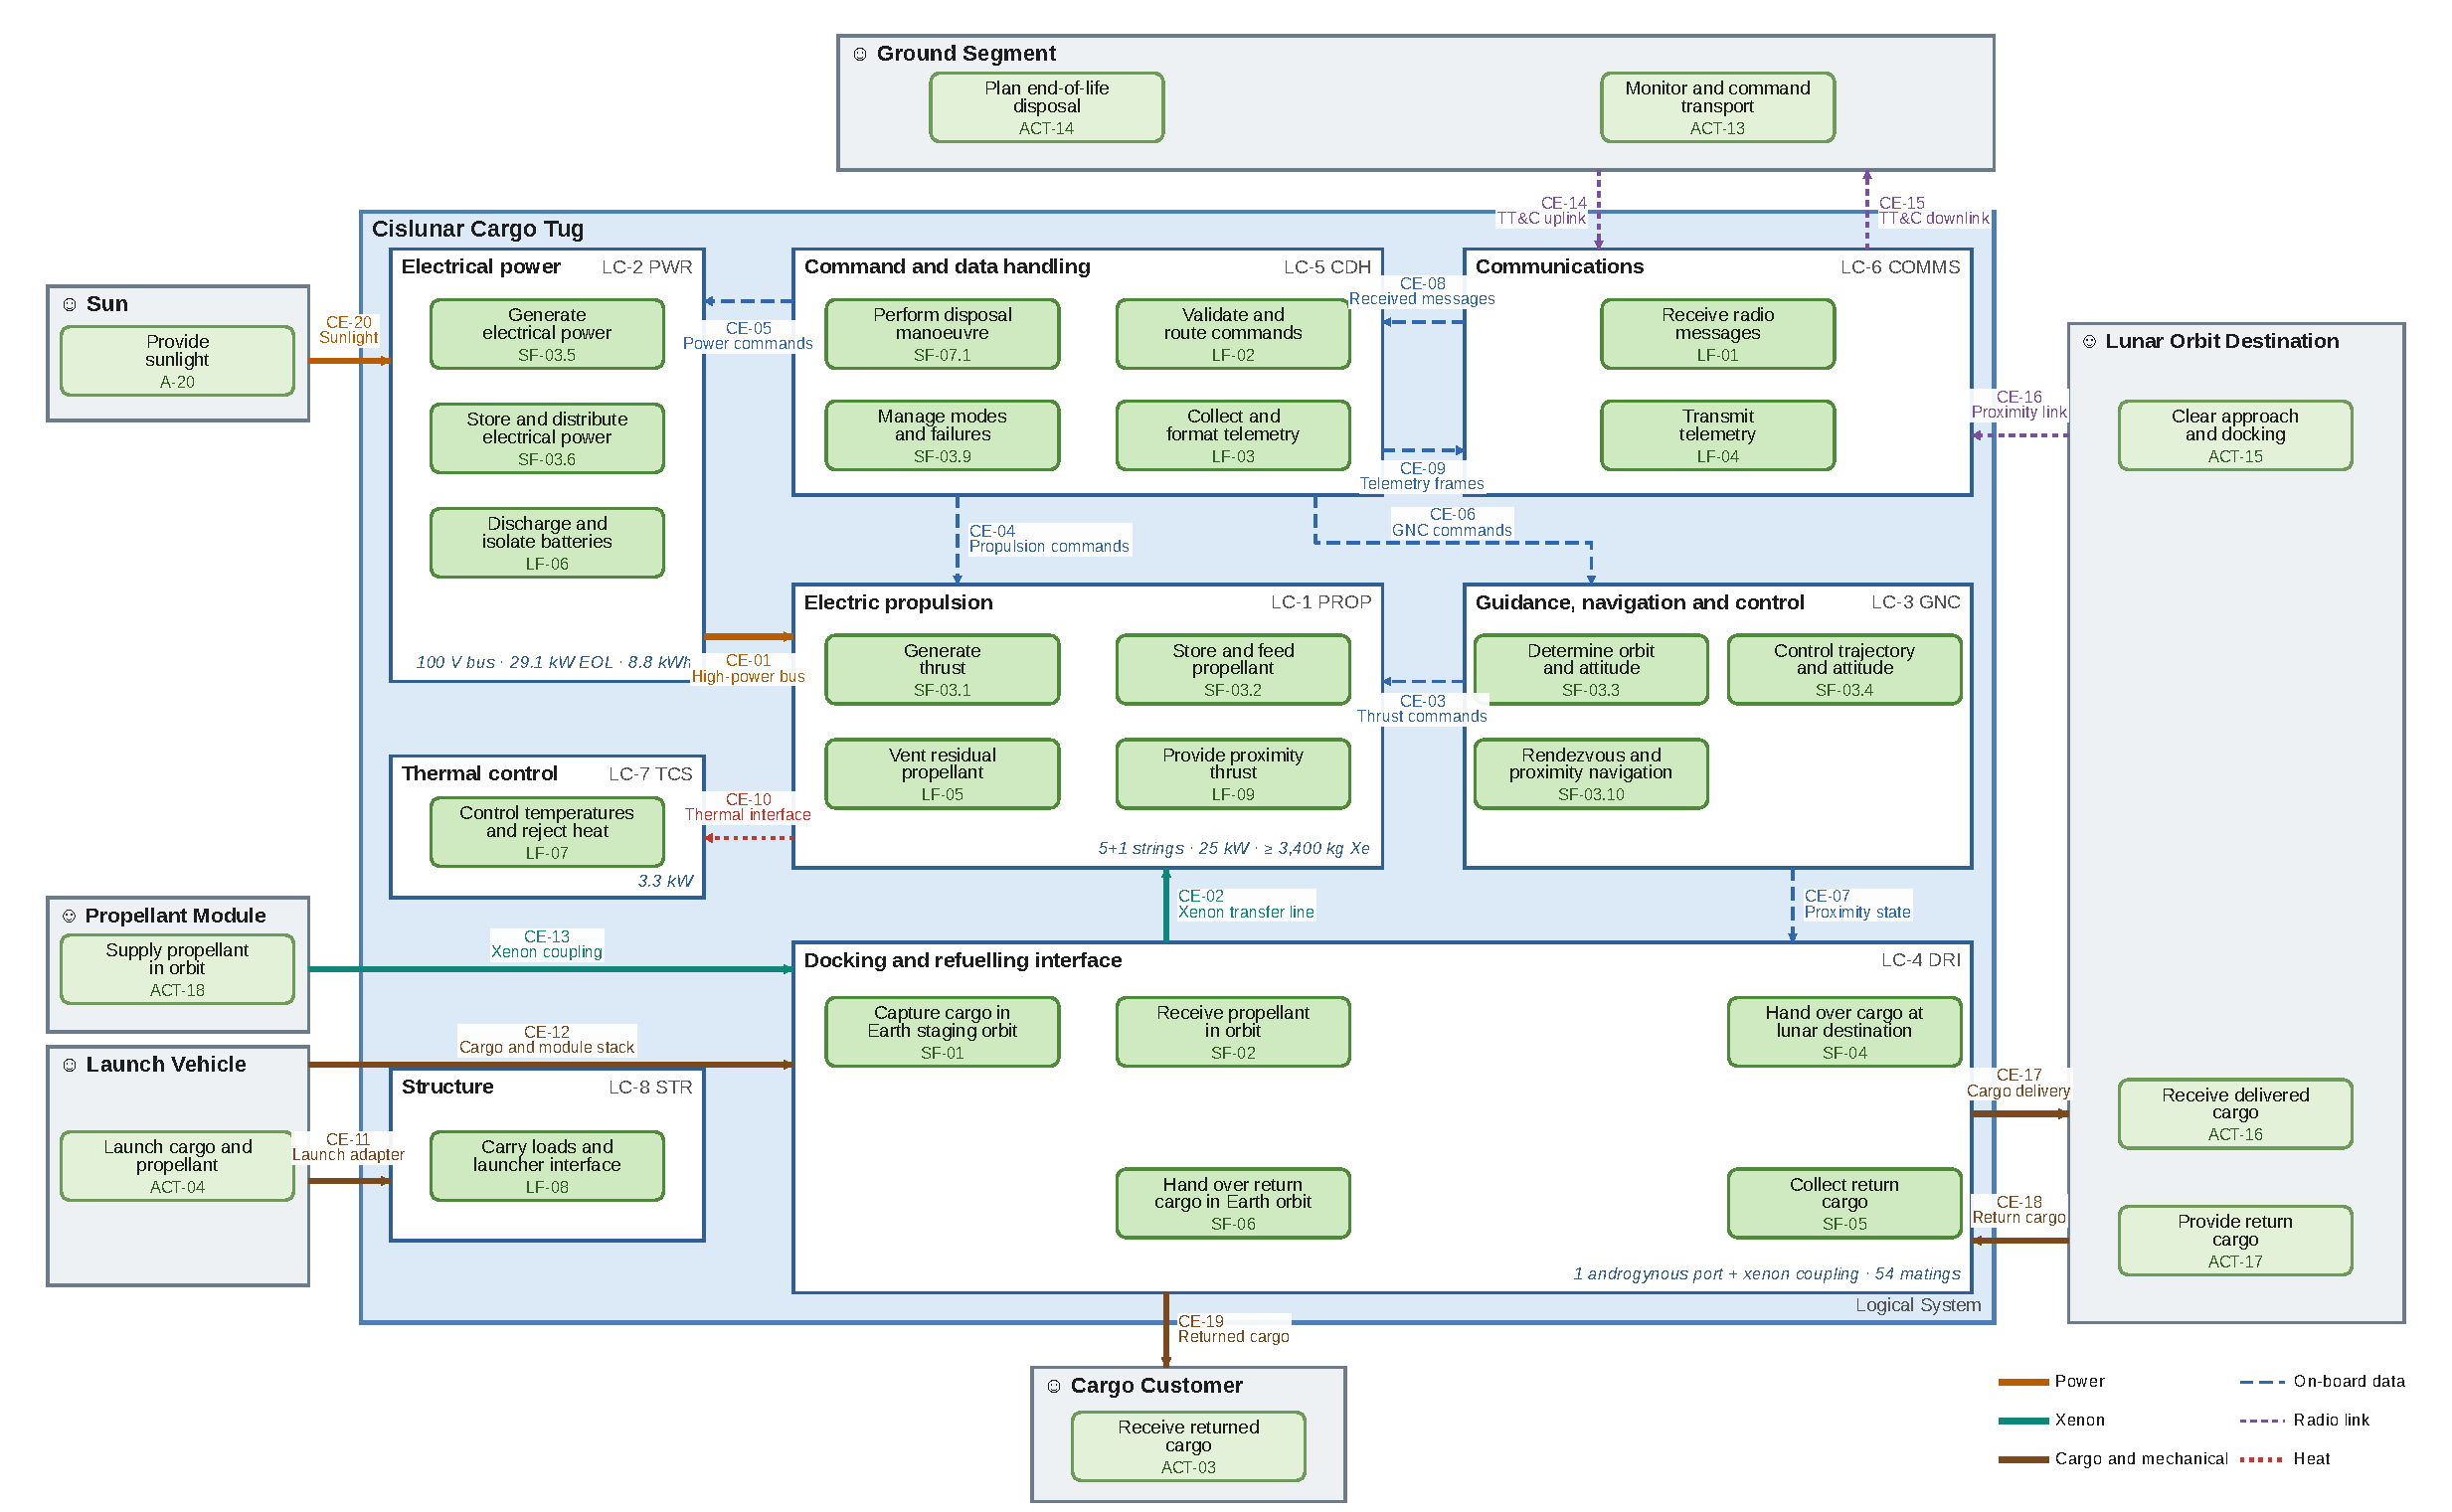
\includegraphics[width=\textheight,height=0.92\textwidth,keepaspectratio]{fig04_logical_architecture.pdf}
\caption{Logical architecture in the layout of a Capella Logical Architecture Blank: the eight logical components with their allocated functions (dark green), the external actors with their functions (light green), and all twenty component exchanges. Italic notes give key figures from the power budget. Report figure drawn from the interface table; the Capella diagrams are in Appendix~\ref{app:capella}.}\label{fig:la}
\end{sidewaysfigure}

\paragraph{Interfaces} The interfaces that drive the design have their own requirements (\id{IR-01} to \id{IR-08}). The high-power bus delivers 25~kW at the PPU inputs from a 100~V regulated bus (TBC) through six individually switchable feeds, one per thruster string, which supports rotation and isolates a failed string (\id{IR-01}, \id{D-23}). The xenon path crosses two interfaces, from the module through the coupling and from the docking interface to the tanks, and must carry 2,550~kg in 21 days (\id{IR-02}). The rule with the largest consequence is \id{IR-04}: each thruster string touches the rest of the tug only through power, xenon and data, which keeps a later propulsion-module exchange possible without redesigning anything else. One definition was also fixed: ``25~kW to the propulsion'' means at the PPU inputs, and the 60\,\% efficiency of the trades is read as PPU (95\,\%) times thruster (63\,\%), which changes no trade-off result (\id{D-22}).

\paragraph{Power budget and sizing} The platform load of each component was estimated in each mode (Figure~\ref{fig:modes}). Docking is the worst mode, with the rendezvous sensors, the capture mechanism and continuous communications all running: 1.11~kW, or 1.33~kW with a 20\,\% margin, inside the 2~kW platform allocation assumed in the system analysis, which is confirmed and kept for sizing (Table~\ref{tab:sizing}).

\begin{figure}[htbp]
\begin{minipage}[t]{0.47\linewidth}\vspace{0pt}\centering
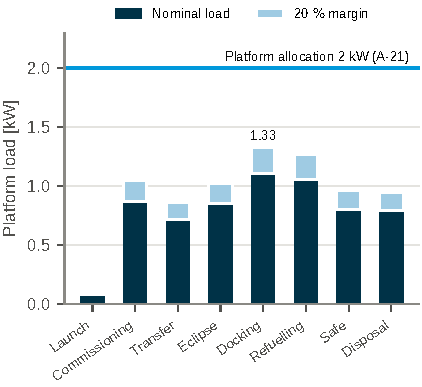
\includegraphics[width=\linewidth]{fig05_power_modes.pdf}
\captionof{figure}{Platform load per mode against the 2~kW allocation. The thruster power (25~kW in Transfer) is not included.}\label{fig:modes}
\end{minipage}\hfill
\begin{minipage}[t]{0.5\linewidth}\vspace{0pt}\small
\captionof{table}{Power chain sizing at the design point.}\label{tab:sizing}
\begin{tabularx}{\linewidth}{@{}Lr@{}}
\toprule
Result & Value \\
\midrule
Longest eclipse in the staging orbit & 2.2~h \\
Design eclipse (\id{A-28}) & 2.5~h \\
Battery, 60\,\% depth of discharge & 8.8~kWh \\
Battery recharge power & 0.69~kW \\
Solar array, end of life & 29.1~kW \\
Solar array, beginning of life & 38.9~kW \\
PPU waste heat & 1.25~kW \\
Heat to reject in Transfer & 3.25~kW \\
Xenon transfer rate (2,537~kg in 21~days) & 121~kg/day \\
\bottomrule
\end{tabularx}
\figsrc{CALC-29 to CALC-39 in \texttt{calculation\_log.md}.}
\end{minipage}
\end{figure}

Three things follow. The array is larger than the trade-offs counted: distribution losses and battery recharge raise the end-of-life need from 27 to 29.1~kW, and radiation degradation over 18 belt crossings per life raises it to about 39~kW at beginning of life, well above the 12--22~kW payload power of Europe's largest telecom platform, Alphabus~\cite{alphabus}. The eclipse is a mission-design constraint as much as a battery size: eclipses longer than 2.5~h are avoided by trajectory phasing rather than carried by a bigger battery (\id{D-26}), as electric orbit-raising tools already do~\cite{electro}, and NRHO eclipses can be avoided altogether~\cite{zimovan}. And thermal control is a real subsystem: about 3.3~kW must be rejected in Transfer, 1.25~kW of it from the PPUs alone.

% =====================================================================
\section{TRL and cost assessment}\label{sec:trl}

\paragraph{Method} Technology readiness follows the ESA TRL handbook and ECSS-E-HB-11A~\cite{trlhandbook,ecsstrl}: a technology is judged against \emph{this} application's requirements, so a product that is flight-proven in one envelope can sit at a low TRL here. The target is TRL~6 at the end of Phase~B1 (about 2030), in line with ESA's practice of reaching TRL~5--6 before mission adoption~\cite{esatrl56}. Mass margins follow the ESA margin philosophy for assessment studies: 5, 10 or 20\,\% by maturity, plus 20\,\% at system level~\cite{esamargins}. Costs stay relative (\id{A-13}): no public figures exist for a European cislunar tug, so the drivers are ranked and measured in launches, hardware counts and mass, not in euros.

\newpage
\subsection{Critical technologies}

A technology is critical when the mission depends on it and it has not yet been demonstrated at the level the mission needs. Five pass that test (Table~\ref{tab:ct}, Figure~\ref{fig:trl}).

\begin{table}[H]\centering\small
\caption{Critical technologies, TRL for this application, and the main evidence.}\label{tab:ct}
\begin{tabularx}{\linewidth}{@{}P{0.95cm}P{3.6cm}cL@{}}
\toprule
ID & Technology & TRL & Evidence and gap \\
\midrule
\id{CT-1} & Long-life 5~kW Hall thruster string, about 50,000~h at 2,100~s & 4 & PPS~5000 qualified and flown (2021--2022), rated about 15,000--20,000~h, catalogue $I_{sp}$ 1,730--2,000~s~\cite{pps5000iac,pps5000cat}. Magnetic shielding is the route to longer life~\cite{hermes}, but no European shielded 5~kW thruster exists beyond the laboratory. \\
\id{CT-2} & Xenon transfer from a passive module, 2,550~kg in 21 days, 54 matings & 5 & ESPRIT couplers developed and ground-tested, not flown; ESPRIT refuels a few times, the tug mates 54 times. \\
\id{CT-3} & 39~kW array and 100~V power control at about 29~kW & 5 & Alphabus flies 100~V buses at 12--22~kW. Arrays of this size in development are US-built, outside \id{SR-24}. Radiation degradation over the life is not characterised. \\
\id{CT-4} & Autonomous capture of a passive cargo stack, androgynous docking, 54 matings & 5 & ATV docked automatically five times with a cooperative target~\cite{atv}; IBDM passed its critical design review~\cite{ibdm}. Passive-stack capture in GTO is not demonstrated. \\
\id{CT-5} & In-orbit propulsion-module exchange (25~kW connector, xenon, data) & 3 & No 25~kW connector has been mated in orbit. Needed only on the module-exchange path. \\
\bottomrule
\end{tabularx}
\end{table}

\begin{figure}[H]
\begin{minipage}[t]{0.45\linewidth}\vspace{0pt}\centering
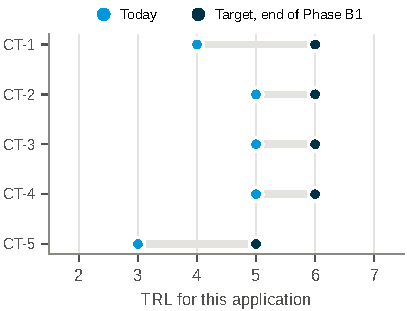
\includegraphics[width=\linewidth]{fig07_trl.pdf}
\captionof{figure}{TRL today and target at the end of Phase~B1. CT-5 targets TRL~5 by then and TRL~6 by PDR.}\label{fig:trl}
\end{minipage}\hfill
\begin{minipage}[t]{0.51\linewidth}\vspace{0pt}\small
Each technology has a Phase~A step to TRL~5 and a Phase~B1 step to TRL~6. For \id{CT-1}: an erosion model and a short wear test of a magnetically shielded 5~kW variant in Phase~A, then a wear test of 5,000~h or more with erosion extrapolated to 50,000~h. For \id{CT-2}: a breadboard transfer at 121~kg/day, then a full-scale ground transfer and a 54-cycle coupling test. For \id{CT-3}: cell radiation tests at the belt-crossing fluence and a 30~kW PCDU breadboard. For \id{CT-4}: hardware-in-the-loop capture tests on a representative passive target.
\end{minipage}
\end{figure}

\subsection{Mass budget}

The dry mass so far was a parametric placeholder from a published tug design~\cite{rimani}: 5.9~t, growing by 25~kg/kW above 18~kW, so 6.08~t at 25~kW. With eight components defined, the mass can now be built bottom-up, each line with its basis and an ESA maturity category (Figure~\ref{fig:mass}). The sourced lines include three ESA large xenon tanks~\cite{lxta}, an IBDM-class docking mechanism~\cite{ibdm}, thrusters and PPUs scaled from AEPS~\cite{aeps}, and an array at 60~W/kg at end of life~\cite{mercer}.

\begin{figure}[htbp]\centering
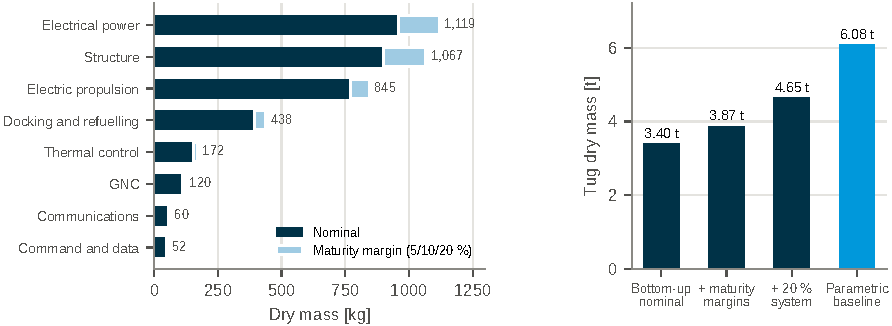
\includegraphics[width=\linewidth]{fig06_mass_budget.pdf}
\caption{Bottom-up dry mass by component with maturity margins (left), and the build-up to the system total compared with the parametric baseline (right).}\label{fig:mass}
\end{figure}

Power and structure carry 56\,\% of the dry mass; the array is the largest single item, and the structure is the largest uncertainty. The bottom-up total, 4.65~t with all margins, is 23\,\% below the parametric value; at that mass the tug would fly 11 round trips instead of 9. The parametric value comes from a complete published design while the bottom-up one still contains own estimates, so 6.08~t stays the baseline and 9 trips is a floor (\id{D-32}). The budget also exposed a missing function: the Hall thrusters give about 1.5~N along one axis, with a slow start-up and a plume that would hit the cargo, so they cannot provide the small six-axis impulses needed in the final metres of a capture. A separate proximity propulsion system was added (\id{PROP-06}, \id{D-31}), with a 60~kg dry allowance; its type and its refuelling are open.

\subsection{Thruster life strategy}

At the design point each of the six strings fires about 8,300~h per round trip. How often they must be replaced depends only on their rated life (Table~\ref{tab:life}). Carrying all spares on board is not an option: at 15,000~h the life consumes 30 string lifetimes.

\begin{table}[htbp]\centering\small
\caption{Propulsion-module exchanges over 9 round trips against rated thruster life.}\label{tab:life}
\begin{tabular}{@{}lrrrr@{}}
\toprule
Thruster set & Rated life per string & One set lasts & Exchanges & Strings used \\
\midrule
5~kW class, 5+1 & 15,000~h & 1 trip & 8 & 54 \\
5~kW class, 5+1 & 20,000~h & 2 trips & 4 & 30 \\
5~kW class, 5+1 & 50,000~h (CT-1 target) & 6 trips & 1 & 12 \\
5~kW class, 5+1 & 75,000~h & 9 trips & 0 & 6 \\
12~kW class at 24~kW, 2+1 & 23,000~h & 3 trips & 2 & 9 \\
\bottomrule
\end{tabular}
\figsrc{The 12~kW class is a US product, in conflict with European sourcing (\id{SR-24}).}
\end{table}

Replacement is affordable in launches: one exchangeable propulsion module (six strings, PPUs, pointing mechanisms and its structure) weighs 380~kg with margin, and every resupply launch has 3.46~t of spare capacity. What it needs is \id{CT-5}, at TRL~3. The decision is therefore to \textbf{run two paths through Phase~A} (\id{D-29}): develop the long-life thruster (\id{CT-1}), which removes almost all exchanges, and the module-exchange interface (\id{CT-5}), which works with today's thruster. The choice is made at the end of Phase~A on the wear-test evidence; meanwhile the architecture keeps the module exchangeable (\id{PROP-05}, \id{IR-08}), which costs little and protects both paths.

\subsection{Cost drivers}

\paragraph{Tug against direct launch} The figure of merit set in the mission definition is cargo delivered against a direct Ariane~64 launch (\id{D-09}). An Ariane~64 can put about 8.6~t into a lunar transfer orbit, and a ballistic lunar transfer reaches NRHO for tens of m/s in about 100--110 days~\cite{parrish}. With 100~m/s budgeted and a 1.2~t expendable carrier (\id{A-36}), a direct launch delivers about 7.1~t of cargo. The tug delivers 5~t per resupply launch, so over 15 years it needs three more launches than direct delivery (Figure~\ref{fig:campaign}).

\begin{figure}[htbp]
\begin{minipage}[t]{0.47\linewidth}\vspace{0pt}\centering
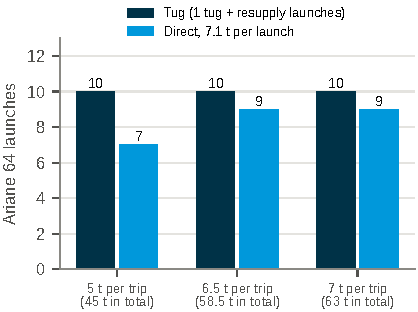
\includegraphics[width=\linewidth]{fig08_launch_campaign.pdf}
\captionof{figure}{Launches over 15 years for the same cargo, tug against direct delivery.}\label{fig:campaign}
\end{minipage}\hfill
\begin{minipage}[t]{0.5\linewidth}\vspace{0pt}\small
This answers the question the study set itself honestly: per launch, direct delivery is better than the baseline tug. The cheapest improvement found is to fill the launcher. Up to 7.29~t per trip still gives 9 round trips, so at about 7~t per trip the tug delivers 40\,\% more cargo for the same launches and the gap to direct delivery falls to one launch (\id{D-30}). The tug can only pay for itself if the expendable carriers of direct delivery cost more than the extra launches plus the tug programme and its consumables. Its other advantages are not counted in launches: it returns cargo, uses any GTO-class launch, and is reusable infrastructure for hub-and-spoke logistics.
\end{minipage}
\end{figure}

\begin{table}[htbp]\centering\small
\caption{Ranked cost drivers.}\label{tab:drivers}
\begin{tabularx}{\linewidth}{@{}cP{3.0cm}LL@{}}
\toprule
Rank & Driver & Evidence & Lever \\
\midrule
1 & One Ariane~64 per trip & 10 launches over the life; 4.5~t of cargo per launch against 7.1~t direct & Fill the launcher: about 7~t per trip keeps 9 trips (\id{D-30}) \\
2 & Thruster life & 30 string lifetimes; 4--8 module exchanges with today's thruster & Long-life thruster or module exchange (\id{D-29}) \\
3 & Power chain beyond the European class & 39~kW array, 29~kW power control; power is 29\,\% of dry mass & Radiation data; 100~V Alphabus heritage (\id{CT-3}) \\
4 & Refuelling consumables & 8 expendable propellant modules of 0.5~t & Larger modules, or a depot later \\
5 & Rendezvous and docking & Docking interface is 11\,\% of dry mass; passive-stack capture & ATV and IBDM heritage; cooperative aids on the cargo \\
6 & Dry mass uncertainty & 4.65~t against 6.08~t: 11 against 9 trips & Bottom-up maturity in Phase~A (\id{D-32}) \\
\bottomrule
\end{tabularx}
\end{table}

% =====================================================================
\section{Conclusions}\label{sec:conclusions}

\paragraph{Findings} A reusable solar-electric tug at 25~kW can deliver 45~t of cargo to NRHO over 15 years in 9 round trips, refuelled from a xenon module launched with each cargo, within the mass limits of one Ariane~64 per trip. It is not limited by power, propellant or launch mass. It is limited by thruster life, which no qualified European thruster meets, and its economics depend on how full each launch is. At the baseline 5~t per trip a direct launch delivers more per launch; at about 7~t per trip the tug comes within one launch of direct delivery while adding return cargo and reusability.

\paragraph{Recommendations for a Phase~A} (1) Baseline about 7~t of cargo per trip, subject to customer demand. (2) Run the two thruster-life paths, a long-life shielded 5~kW thruster and a propulsion-module exchange interface, with a down-select at the end of Phase~A. (3) Start radiation testing of array cells early, because the end-of-life to beginning-of-life ratio sets the size of the largest single item. (4) Mature the bottom-up mass budget, especially the structure, to converge with the parametric value. (5) Define the proximity propulsion system and its refuelling. (6) Replace the relative cost drivers with a parametric cost model once a cost basis is available.

\paragraph{Limitations} The delta-v per leg is held independent of thrust, transfers are not optimised trajectories, the costs are relative only, the platform loads and several mass lines are own estimates, and the ground segment and physical architecture are out of scope. None of the results has been independently reviewed. These limits are acceptable for the purpose of the study, which is learning, but they would not be for a real Phase~A.

\paragraph{Lessons from the process} Four things stood out while doing the work. A requirement on a step-function output such as a trip count needs a margin on its inputs, not only a nominal value. Each Arcadia layer found something the previous one could not: the system analysis turned life into a throughput requirement, the logical architecture exposed a missing navigation input to capture and the heat that must be rejected, and the mass budget exposed the missing proximity propulsion. Fixing a reference comparison at the start (the direct launch) kept the study honest about where the concept's advantage really lies. And keeping every assumption, decision and calculation under an identifier made it possible to change a value late and see everything it touched.

% =====================================================================
\begin{thebibliography}{99}\small
\setlength{\itemsep}{1pt}
\bibitem{strategy2040} ESA, \emph{ESA Strategy 2040} (in-depth version), 2025. \url{https://esamultimedia.esa.int/docs/corporate/ESA_Strategy_2040_InDepth.pdf}
\bibitem{explore2040} ESA, \emph{Explore2040: The European Exploration Strategy}, 2024. \url{https://esamultimedia.esa.int/docs/HRE/Explore_2040.pdf}
\bibitem{techvision} ESA, \emph{Technology 2040: A Vision for the European Space Agency}, 2025. \url{https://esamultimedia.esa.int/docs/technology/Technology_2040.pdf}
\bibitem{repo} \studyauthor, \emph{cislunar-tug-study} repository: study documents, Capella model, requirement tables and Python model. \url{\repourl}
\bibitem{arcadia} Eclipse Capella, ``Arcadia: a model-based engineering method''. \url{https://mbse-capella.org/arcadia.html}
\bibitem{loghry} C.~Loghry et al., ``LEO to GEO (and Beyond) Transfers using High Power Solar Electric Propulsion'', IEPC 2017. \url{https://ntrs.nasa.gov/api/citations/20180000689/downloads/20180000689.pdf}
\bibitem{estublier} D.~Estublier et al., ``Electric Propulsion on SMART-1: A Technology Milestone'', \emph{ESA Bulletin} 129. \url{https://www.esa.int/esapub/bulletin/bulletin129/bul129e_estublier.pdf}
\bibitem{rimani} J.~Rimani, C.~A.~Paissoni, N.~Viola, G.~Saccoccia, J.~Gonzalez del Amo, ``Multidisciplinary mission and system design tool for a reusable electric propulsion space tug'', \emph{Acta Astronautica} 175 (2020) 387--395. \url{https://iris.polito.it/retrieve/handle/11583/2837701/379000}
\bibitem{mcguire2024} M.~L.~McGuire et al., ``Application of Solar Electric Propulsion to the Low Thrust Lunar Transit of the Gateway Power and Propulsion Element'', IEPC 2024. \url{https://ntrs.nasa.gov/api/citations/20240007012/downloads/IEPC24_358_v2.pdf}
\bibitem{whynrho} NASA, ``Why NRHO: The Artemis Orbit'', Architecture Concept Review white paper, 2022. \url{https://www.lpi.usra.edu/lunar/artemis/resources/WhitePaper_2023_WhyNRHA-TheArtemisOrbit.pdf}
\bibitem{gatewaypause} The Register, ``NASA abandons Lunar Gateway plans for base on Lunar surface'', 24 March 2026. \url{https://www.theregister.com/offbeat/2026/03/24/nasa-abandons-lunar-gateway-plans-for-base-on-lunar-surface/5225207}
\bibitem{ariane} ArianeGroup, ``Number crunching: Ariane 62 and Ariane 64''. \url{https://www.ariane.group/en/news/number-crunching-ariane-6-ariane-62-and-ariane-64/}
\bibitem{ohbesprit} ESA, ``Gateway: Lunar View'' (formerly the ESPRIT Refuelling Module). \url{https://www.esa.int/Science_Exploration/Human_and_Robotic_Exploration/Gateway_Lunar_View}
\bibitem{radke} C.~Radke et al., ``Gateway to the Future: Lessons Learned in Development of the Refueling Systems for NASA's First Lunar Space Station'', 75th International Astronautical Congress, Milan, 2024. \url{https://ntrs.nasa.gov/citations/20240011961}
\bibitem{alphabus} ESA, ``Alphabus: An Extended European Capability''. \url{https://resilience.esa.int/archives/news/alphabus-extended-european-capability}
\bibitem{electro} J.~C.~Bastante, P.~Peñarroya, ``ELECTRO: A SW Tool for the Electric Propulsion Trajectory Optimisation'', ICATT 2018. \url{https://indico.esa.int/event/224/papers/3875/files/204-ICATT-2018_Bastante_ELECTRO.pdf}
\bibitem{zimovan} E.~M.~Zimovan-Spreen, K.~C.~Howell, D.~C.~Davis, ``Eclipse Avoidance in Dynamical Structures Nearby NRHOs in a Higher-Fidelity Model'', AAS 20-562. \url{https://engineering.purdue.edu/people/kathleen.howell.1/Publications/Conferences/2020_AAS_SprHowDav.pdf}
\bibitem{trlhandbook} ESA, ``Technology Readiness Levels (TRL)''. \url{https://www.esa.int/Enabling_Support/Space_Engineering_Technology/Shaping_the_Future/Technology_Readiness_Levels_TRL}
\bibitem{ecsstrl} ECSS, \emph{ECSS-E-HB-11A Technology readiness level (TRL) guidelines}, 2017. \url{https://ecss.nl/home/ecss-e-hb-11a-technology-readiness-level-trl-guidelines-1-march-2017/}
\bibitem{esatrl56} ESA, ``Technology development in support of future science missions''. \url{https://sci.esa.int/web/sci-ft/-/50034-technology-development-in-support-of-future-science-missions}
\bibitem{esamargins} ESA, \emph{Margin philosophy for science assessment studies}, SRE-PA/2011.097, issue~1.3. \url{https://sci.esa.int/documents/34375/36249/1567260131067-Margin_philosophy_for_science_assessment_studies_1.3.pdf}
\bibitem{pps5000iac} Safran, PPS~5000 life test and qualification, IAC-21 abstract. \url{https://p.iafastro.directory/iac/paper/id/64241/abstract-pdf/IAC-21,C4,5,5,x64241.brief.pdf}
\bibitem{pps5000cat} satcatalog, ``PPS5000''. \url{https://www.satcatalog.com/component/pps5000/}
\bibitem{hermes} J.~D.~Frieman et al., ``Completion of the Long Duration Wear Test of the NASA HERMeS Hall Thruster''. \url{https://ntrs.nasa.gov/api/citations/20190031949/downloads/20190031949.pdf}
\bibitem{atv} CNES, ``ATV''. \url{https://cnes.fr/en/projects/atv}
\bibitem{ibdm} ``International Berthing and Docking Mechanism'', Wikipedia. \url{https://en.wikipedia.org/wiki/International_Berthing_and_Docking_Mechanism}
\bibitem{lxta} ESA ARTES, ``L-XTA: Large Xenon Tank Assembly''. \url{https://resilience.esa.int/archives/projects/l-xta-large-xenon-tank-assembly}
\bibitem{aeps} NASA, ``12-kW Advanced Electric Propulsion System Hall Current Thruster Qualification and Production Status'', 2025. \url{https://ntrs.nasa.gov/citations/20250003901}. The thruster and power processing unit masses per kW also use the L3Harris AEPS spec sheet (2023), which is no longer online.
\bibitem{mercer} C.~Mercer, ``Advanced Solar Arrays'', NASA GRC, 2014. \url{https://discovery.larc.nasa.gov/pdf_files/02-AdvSolrArry-CMercer-2.pdf}
\bibitem{parrish} N.~L.~Parrish et al., ``Ballistic Lunar Transfers to Near Rectilinear Halo Orbit: Operational Considerations''. \url{https://ntrs.nasa.gov/api/citations/20200011549/downloads/20200011549.pdf}
\bibitem{mcguire2021} M.~L.~McGuire et al., ``Overview of the Lunar Transfer Trajectory of the Co-Manifested First Elements of NASA's Gateway'', AAS 21-697, 2021. \url{https://ntrs.nasa.gov/api/citations/20210019116/downloads/AAS_McGuire_LunarTransferTraj_v8.pdf}
\end{thebibliography}

% =====================================================================
\appendix
\newpage
\section{Assumption and decision registers}\label{app:registers}

Every input that is not taken directly from a source is an assumption, and every choice is a decision. Both registers continue across the phases; the value shown is the current one. Full bases are in the phase documents of the repository.

{\small
\setlength{\LTpre}{2pt}\setlength{\LTpost}{6pt}
\begin{longtable}{@{}P{1.0cm}P{4.3cm}P{9.8cm}@{}}
\caption{Assumption register.}\label{tab:assumptions}\\
\toprule
ID & Assumption & Value and basis \\
\midrule\endfirsthead
\toprule ID & Assumption & Value and basis \\ \midrule\endhead
\bottomrule\endfoot
\id{A-01} & Cargo per outbound trip & 5~t (sensitivity 3--8.5~t); close to the 5.4~t of Rimani et al. \\
\id{A-02} & Return cargo & Up to 0.5~t per trip (Explore2040 return need) \\
\id{A-03} & Life & 15 years; trip count is an output of the power trade (9 at 25~kW) \\
\id{A-04} & Staging orbit & GTO-class (SMART-1, Rimani et al., Gateway PPE) \\
\id{A-05} & Destination & NRHO, period about 6.6 days; low lunar orbit excluded \\
\id{A-06} & Delta-v per leg & 2.4~km/s + 10\,\% = 2.64~km/s; sensitivity 3.1~km/s \\
\id{A-07} & Return-leg delta-v & Equal to outbound \\
\id{A-08} & Propulsion & Hall thrusters on xenon, 2,000--2,700~s \\
\id{A-09} & Supply & One Ariane~64 to GTO per trip carries the cargo and the next trip's xenon \\
\id{A-10} & Propellant and dry mass & About 2.5~t of xenon per trip; 5.9~t dry mass placeholder (Rimani et al.) \\
\id{A-11} & Schedule & Phase~B1 about 2029--2030; operations about 2036--2038 \\
\id{A-12} & Disposal & Heliocentric after a lunar flyby, or controlled lunar impact \\
\id{A-13} & Cost & Relative cost drivers only (public information limit) \\
\id{A-14} & Return to the ground & Out of scope (Earth return vehicles) \\
\id{A-15} & Propellant route & Same Ariane~64 as the cargo \\
\id{A-16} & Ground segment & One Ground Operations entity \\
\id{A-17} & Reference thrust, duty cycle & 1.05~N at 2,100~s (about 18~kW), superseded by \id{D-16}; 85\,\% thrusting duty cycle (Gateway PPE: 319 of 383 days) \\
\id{A-18} & End operations & 60 days per round trip \\
\id{A-19} & Thruster total efficiency & 60\,\%, read as PPU $\times$ thruster (\id{D-22}) \\
\id{A-20} & Sun as actor & Source of sunlight in the system analysis \\
\id{A-21} & Platform power & 2~kW allocation, confirmed by the power budget \\
\id{A-22} & Communication range & 450,000~km (Earth--Moon distance plus NRHO apolune) \\
\id{A-23} & Added dry mass per kW & 25~kg/kW above 18~kW (swept 15--40) \\
\id{A-24} & European thruster class & 5~kW, about 15,000~h rated life (PPS~5000 catalogue) \\
\id{A-25} & Propellant module dry mass & About 0.5~t (20\,\% of the xenon load) \\
\id{A-26} & Xenon transfer time & At most 21 days (ESPRIT: up to about 3 weeks~\cite{radke}) \\
\id{A-27} & Spare thruster policy & Rotation: the N+1 units take turns \\
\id{A-28} & Design eclipse & 2.5~h (2.2~h calculated at GTO-class apogee) \\
\id{A-29} & PPU and thruster efficiency & 95\,\% (ESA ARTES high-power PPU breadboard) and 63\,\% \\
\id{A-30} & Power margin, distribution & 20\,\% on estimates; 95\,\% distribution efficiency \\
\id{A-31} & Battery & 60\,\% depth of discharge, 95\,\% efficiency (Li-ion, a few thousand cycles) \\
\id{A-32} & Array degradation & End-of-life to beginning-of-life ratio 0.75 (TBC by dose analysis) \\
\id{A-33} & Platform loads & Per component and mode, each with its basis (\texttt{power\_budget.toml}) \\
\id{A-34} & Mass lines & Public sources where they exist, own estimates otherwise (\texttt{mass\_budget.toml}) \\
\id{A-35} & Mass margins & 5/10/20\,\% by maturity, 20\,\% system (ESA SRE-PA/2011.097) \\
\id{A-36} & Direct-launch alternative & 8.6~t to lunar transfer orbit, 100~m/s, 300~s, 1.2~t carrier (swept 0.8--1.6~t) \\
\id{A-37} & TRL target & TRL~6 at the end of Phase~B1 \\
\id{A-38} & PPS~5000 life, sensitivity & 20,000~h (baseline stays 15,000~h) \\
\end{longtable}

\begin{longtable}{@{}P{1.0cm}P{14.4cm}@{}}
\caption{Decision register.}\label{tab:decisions}\\
\toprule
ID & Decision \\
\midrule\endfirsthead
\toprule ID & Decision \\ \midrule\endhead
\bottomrule\endfoot
\id{D-01} & Concept fixed by the ESA 2040 documents: reusable, refuellable solar-electric tug \\
\id{D-02} & Staging orbit GTO-class rather than LEO \\
\id{D-03} & Destination NRHO, as a staging orbit rather than a Gateway commitment \\
\id{D-04} & Hall thrusters on xenon \\
\id{D-05} & 5~t out, 0.5~t back, repeated round trips over 15 years \\
\id{D-06} & Operational analysis solution-neutral: \emph{Cislunar Cargo Transport} stands for the tug \\
\id{D-07} & Need written as ``replenish transport propellant in orbit'' \\
\id{D-08} & Returning cargo extends delivery \\
\id{D-09} & The tug is judged against a direct Ariane~64 launch to the Moon \\
\id{D-10} & Low lunar orbit excluded; the tug stops at NRHO \\
\id{D-11} & System of interest is the tug; ground segment is an actor \\
\id{D-12} & Space safety authority is not a system-analysis actor \\
\id{D-13} & Return cargo stays an optional capability \\
\id{D-14} & Flow-down to propulsion, power and the docking and refuelling interface \\
\id{D-15} & Requirements in traceability tables, IDs in the Capella element descriptions \\
\id{D-16} & Electric propulsion power 25~kW (1.46~N at 2,100~s) \\
\id{D-17} & Refuelling by fluid transfer from a co-launched propellant module \\
\id{D-18} & Thruster wear-out is the top risk; propulsion-module swap kept as growth path \\
\id{D-19} & Propellant supplier becomes a passive propellant module; one rendezvous per trip \\
\id{D-20} & 5+1 thrusters of the 5~kW European class (baseline); 2+1 of the 12~kW class at 24~kW (option) \\
\id{D-21} & Eight logical components; flowed-down subsystem boundaries kept \\
\id{D-22} & Thruster power defined at the PPU inputs \\
\id{D-23} & Six thruster strings, one PPU each, on individually switchable feeds \\
\id{D-24} & Thruster strings connect only through power, xenon and data \\
\id{D-25} & 100~V regulated high-power bus (TBC) \\
\id{D-26} & Eclipses longer than 2.5~h avoided by trajectory phasing \\
\id{D-27} & All radio traffic through communications; command and data handling validates and routes \\
\id{D-28} & Mass budget built bottom-up in the TRL and cost assessment \\
\id{D-29} & Thruster life: two paths through Phase~A (long-life thruster, module exchange) \\
\id{D-30} & Recommend about 7~t of cargo per trip for Phase~A (study keeps 5~t) \\
\id{D-31} & Add proximity propulsion with a mass allowance \\
\id{D-32} & Parametric 6.08~t stays the baseline dry mass; bottom-up 4.65~t is an upside \\
\id{D-33} & Five critical technologies, each with a Phase~A and Phase~B1 step to TRL~6 \\
\end{longtable}
}

% =====================================================================
\newpage
\section{Capella diagrams}\label{app:capella}

The Capella model is in the repository (\texttt{capella/CislunarCargoTug}), with every diagram as an image file in \texttt{capella/diagrams/}. It covers the operational analysis, the system analysis and the logical architecture; the Operational Architecture Blank is Figure~\ref{fig:oab}. Each element carries its study ID (ACT-, INT-, SF-, LF-, FE-, CE-) in its name, so the diagrams can be read against the tables in this report.

\capellafig{OA-1_OCB}{Operational Capabilities Blank: the five operational capabilities and the entities involved in each. \guillemotleft i\guillemotright: include; \guillemotleft e\guillemotright: extend.}{fig:oa1}
\capellafig{OA-4_OAIB}{Operational Activity Interaction Blank: the twenty operational activities and nineteen interactions, without the entities. Red: physical; dashed blue: information.}{fig:oa4}
\capellafig{OA-3_OES_SC-1}{Operational Entity Scenario SC-1: one reusable round trip, repeated about nine times over the 15-year life at the 25~kW design point.}{fig:oa3}
\capellafig{SA-1_MCB}{Missions and Capabilities Blank: the system mission, its four capabilities and the actors involved in each.}{fig:sa1}
\capellafig{SA-2_SAB}{System Architecture Blank: the tug, its six actors, 17 leaf functions and 24 functional exchanges. Red: physical; dashed blue: information.}{fig:sa2}
\capellafig{SA-3_SAB_chains}{The same architecture with the three functional chains highlighted: FC-1 cargo delivery (purple), FC-2 refuelling (green), FC-3 disposal (red).}{fig:sa3}
\capellafig{SA-4_MSM}{Mode state machine: the seven modes and fourteen transitions, with their guards in brackets.}{fig:sa4}
\capellafig{LA-1_LCBD}{Logical Component Breakdown: the eight logical components of the tug.}{fig:la1}

\begin{sidewaysfigure}\centering
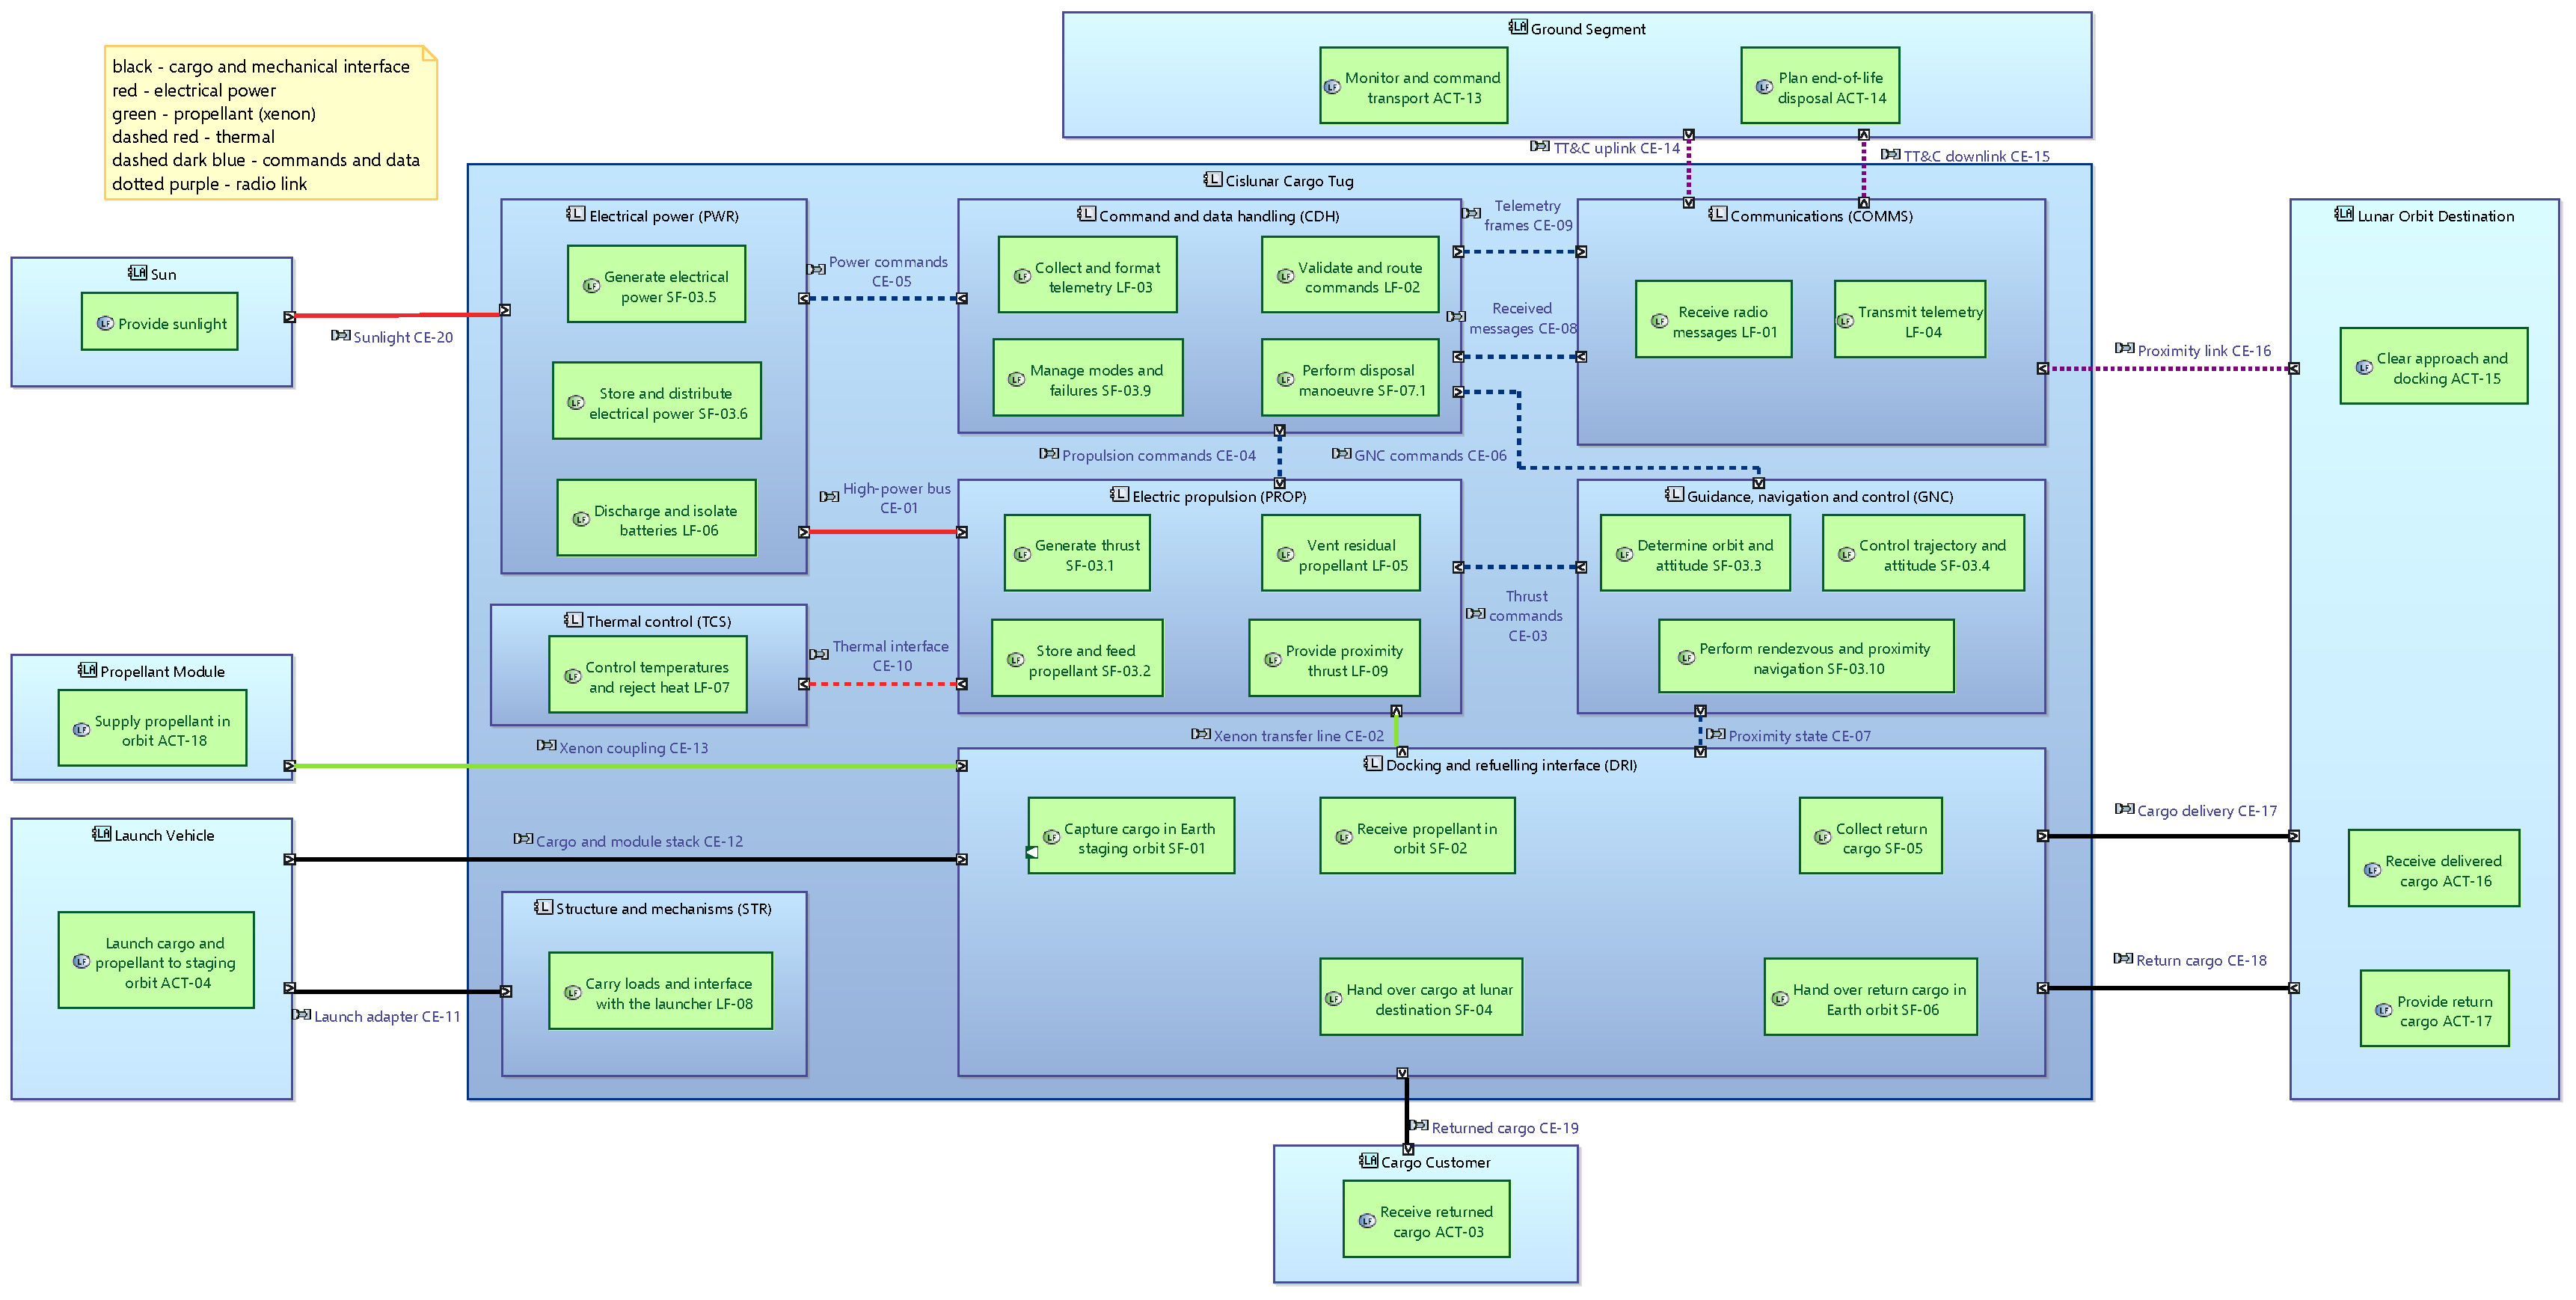
\includegraphics[width=\textheight,height=0.9\textwidth,keepaspectratio]{capella/LA-2_LAB.pdf}
\caption{Logical Architecture Blank: the eight logical components with their allocated functions, the external actors and the twenty component exchanges.}\label{fig:la2}
\end{sidewaysfigure}

\capellafig{LA-3_LAB_FC-2}{Logical Architecture Blank for propulsion and refuelling: the xenon path from the propellant module to the thrusters, with the power, thermal and command interfaces around it.}{fig:la3}

% =====================================================================
\clearpage
\section{Reproducing the results}\label{app:repro}

\sloppy
Everything in this report can be regenerated from the repository~\cite{repo}.
\begin{enumerate}
  \item \textbf{Model.} In \texttt{model/}: \texttt{pip install -e ".[plot,dev]"}, then \texttt{cislunar-tug run} writes all result tables and the calculation log to \texttt{model/results/baseline/}; \texttt{pytest} runs the 73 tests. Parameters, each with unit, reference and source, are in \texttt{model/config/}.
  \item \textbf{Figures.} \texttt{python report/figures/make\_figures.py} redraws every report figure from the result tables, the requirement tables and the study documents.
\end{enumerate}
The calculation log has 53 entries, 50 calculations and 3 validations against published cases: 23 agree with a value in the mission definition and 30 are new.

\end{document}
